% 1977 年吉林卷第 3 题：港口暗礁轨迹示意——圆内弦 AB、圆周角顶点 M（在圆上）
% 与圆外船只 S，S、M、B 共线，另画 SA 与 AM（按源卷第 2 页布局：S 在上、AB 在下）
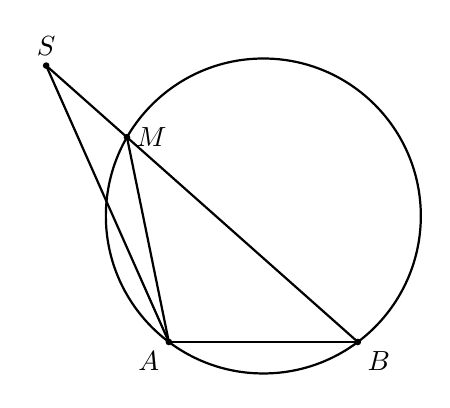
\begin{tikzpicture}[scale=1.0]
  \draw[thick] (0,0) circle (2);
  \coordinate (A) at (-1.2,-1.6);
  \coordinate (B) at (1.2,-1.6);
  \coordinate (M) at (-1.732,1);
  \coordinate (S) at (-2.758,1.91);
  \draw[thick] (S)--(B);
  \draw[thick] (S)--(A);
  \draw[thick] (A)--(B);
  \draw[thick] (A)--(M);
  \fill (A) circle (1.2pt) node[below left] {$A$};
  \fill (B) circle (1.2pt) node[below right] {$B$};
  \fill (M) circle (1.2pt) node[right] {$M$};
  \fill (S) circle (1.2pt) node[above] {$S$};
\end{tikzpicture}
